\documentclass[a4paper,11pt,openright,openbib]{article}
\usepackage[portuges]{babel}
\usepackage[T1]{fontenc}
\usepackage{ae}
\usepackage[utf8]{inputenc}
\usepackage[pdftex]{graphicx}
\usepackage{url}
\usepackage{listings}
\usepackage{verbatim}
\usepackage{enumerate}
\usepackage[a4paper, pdftex, bookmarks, colorlinks, linkcolor=black, urlcolor=blue]{hyperref} 
\usepackage[a4paper,left=2.5cm,right=2.5cm,top=3.5cm,bottom=3.5cm]{geometry}
\usepackage{colortbl}
\usepackage[margin=10pt,font=small,labelfont=bf]{caption}
\usepackage{mdwlist}


\setlength{\parindent}{0cm}
\setlength{\parskip}{2pt}




\title{
	\large{
\includegraphics[width=0.3\textwidth]{../../../report-template/UM.jpg}} \\
	\large{Universidade do Minho}  \\
	\large{Mestrado em Engenharia Informática}  \\
	\large{Engenharia de Linguagens}  \\
	\large{Engenharia Gramatical - Grupo 1}  \\	
	\large{\textbf{Resolução das Fichas 3 e 5}} \\
	\large{Ano Lectivo de 2012/2013} \\
	\date{\today}
}

\author{	
	\begin{tabular}[t]{c c}      
        pg22820 - \textbf{António Silva} \\        
		pg22781 - \textbf{Rui Brito} \\   				
	\\ 
	\end{tabular}
}

\begin{document}

\maketitle


\pagestyle{headings}
\pagenumbering{arabic}
\newpage
\tableofcontents
\newpage
%Ele disse que o relatório não precisa de ser uma coisa muito complexa. Essencialmente é para explicar o que foi feito,
%e no caso de haver respostas a dar, serem dadas aqui.
\section{Introdução}
Este primeiro trabalho de \emph{Engenharia Gramatical} de avaliação, da Unidade Curricular de Especialização 
\emph{Engenharia de Linguagens}, consiste na realização da ficha 3 e 5 disponiblizadas no Blackboard.
\section{Ficha 3}
\subsection{Composição do Corpo}
Para escrever uma gramática tradutora, foi necessário completar a informação sobre o corpo. Assim incialmente o corpo da
factura era um conjunto de linhas, em que cada linhas era \emph{'(' codartigo ',' designacao ',' pvu ',' quantidade ')'}.
Depois para suportar o pedido da alínea c, cada linhas passou a ser somente \emph{'(' codartigo ',' quantidade ')'}.
\subsection{Código Java}
Para conseguirmos saber os totais dos produtos, com várias facturas (sendo que cada factura possuia um id alfanumérico),
foi criado um \emph{hashmap} para associar a cada id de factura uma lista de valores, que era o total de cada linha
da factura. No final, é possível apresentar o o total de cada linha em cada factura e ainda o tal de cada factura (que 
mais não é que a soma dos totais das linhas).
Para se obter o Preço Unitário, que a pedido da alínea c) deveria já ter sido indicado no ínicio, foi também criada um
\emph{hashmap} com a correspondência entre o código do produto e os seus atributos (guardados numa classe). Assim, por
cada linha só era necessário obter o PVU através do código do artigo, e multiplicá-lo pela quantidade.
\subsection{Exemplo de Input}
\begin{verbatim}
a1 "xpto" 3.6 50
a2 "outro" 1 60.5
a3 "mais um" 4.99 4
---

f1
	"Nome 1" "NIF 1" "Morada 1" "NIB 1"
	"Nome 2" "NIF 2" "Morada 2"
	(a1,5) (a3,2)
;

f2
	"Nome 3" "NIF 3" "Morada 3" "NIB 3"
	"Nome 4" "NIF 4" "Morada 4"
	(a2,9.5) (a1,5) (a3,2)
;

f3
	"Nome 5" "NIF 5" "Morada 5" "NIB 5"
	"Nome 6" "NIF 6" "Morada 5"
	(a2,2.25)
.
\end{verbatim}

\section{Ficha 5} % (fold)
\label{sec:ficha_5}

\subsection{Exemplo de frase válida e Árvore de Derivação}

Um exemplo rudimentar de frase válida seria: 
\begin{verbatim}
[ REGISTO id1122 LIVRO "nome_livro" ("nome_autor") "nome_editora" 2010 BGUM 
EXISTENCIAS LOCAL "Braga" ( cb54433231 ; PERMANENTE ) ]
\end{verbatim}

A árvore de derivação corresponde seria como se segue:

\begin{figure}[!htb]
	\begin{center}
		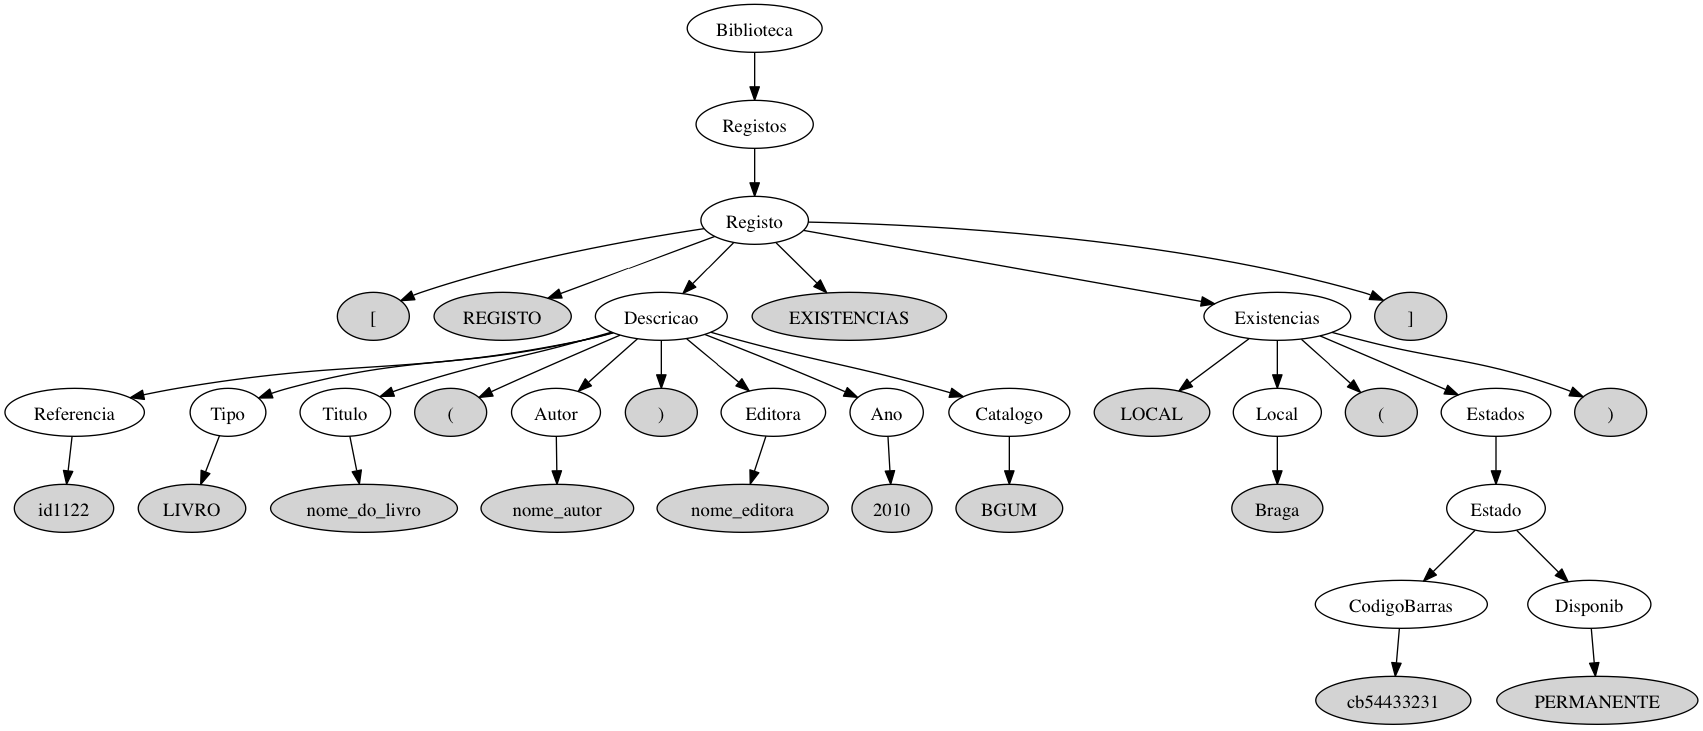
\includegraphics[width=\textwidth,keepaspectratio]{../ficha5/g.png}
	\end{center}	
	\caption{\label{parse_tree}Árvore de Derivação}
\end{figure}

\small{Imagem em maior detalho na figura \ref{parse_tree_ap}}

\subsection{Lista de Autores}
Para permitir uma lista de autores ao contrário de apenas um, basta extender a produção dez.
Ficaria, então, algo como segue abaixo:

\begin{verbatim}
	p10: Autores --> Autor
	p11:           | Autores ',' Autor
\end{verbatim}

\subsection{Recursividade à esquerda para Recursividade à direita}

Recursividade à esquerda:
\begin{verbatim}
	p1: Registos --> Registo
	p2:            | Registos ',' Registo
\end{verbatim}

O que transformado para recursividade à direita (assumindo a notação eBNF):

\begin{verbatim}
	p1: Registos --> Registo
	p2:            | Registo ',' Registos
\end{verbatim}

As diferenças quando à árvore de derivação são apresentadas a seguir:

\begin{figure}[!htb]
	\begin{center}
		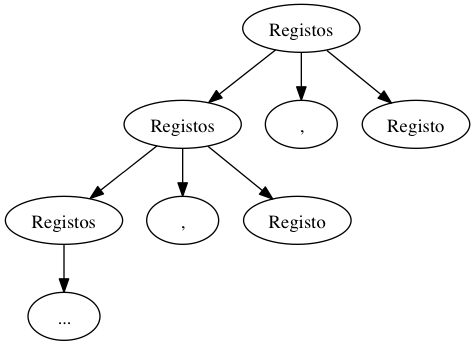
\includegraphics[scale=.5]{../ficha5/lr.png}
	\end{center}	
	\caption{\label{lrec}Recursivo à esquerda}
\end{figure}

\begin{figure}[!htb]
	\begin{center}
		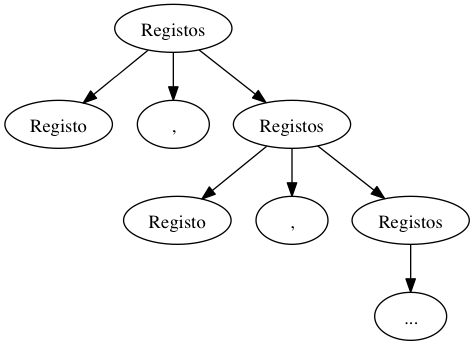
\includegraphics[scale=.5]{../ficha5/rr.png}
	\end{center}	
	\caption{\label{lrec}Recursivo à direita}
\end{figure}

\section{Gramática Tradutora} % (fold)
\label{sec:gram_tica_tradutora}

\begin{verbatim}
	grammar ficha5;

options{
	k=2;
	language=Java;
}

@header{
	import java.util.TreeSet;
}

@members{
	int numRegistos = 0;
	int numLivros = 0;
	String refReg = null;
	
	int reservados = 0;
	int permanentes = 0;
	int estante = 0;
	
	Boolean isBook = false;
	
	TreeSet<String> bookNames = new TreeSet<String>();
	TreeSet<String> refs = new TreeSet<String>();
}

biblioteca 
@after{
System.out.println ("Livros Reservados: " + reservados);
System.out.println ("Livros Permanentes: " + permanentes);
System.out.println ("Livros em Estante: " + estante);

System.out.println("=== Livros ===");
for (String s : bookNames) {
	System.out.println(s);
}

}
	:	registos
	;
	
registos 
	:	registo{numRegistos++;} (',' registo{numRegistos++;})*
	;

registo
@after {
	System.out.println(refReg + ": " + numLivros);
	numLivros = 0;
	refReg = null;
}
	:	'[ REGISTO ' descricao ' EXISTENCIAS ' existencias ']'
	;
	
descricao
	:	referencia {refReg = $referencia.text; 
	           if(!refs.add($referencia.text)){
	                    System.out.println("Referencia ja existente: " + $referencia.text);} 
	                    } 
	                    tipo titulo {if(isBook) {
	                          bookNames.add($titulo.text);isBook = false;}
	                          } '(' autores ')' editora ano catalogo
	;
	
autores
	:	autor (',' autor)*
	;
	
referencia
	:	ID
	;
	
tipo:	'LIVRO' {numLivros++; isBook = true;}
	|	'CDROM'
	|	'OUTRO'
	;

titulo
	:	STRING
	;

autor
	:	STRING
	;

editora
	:	STRING
	;
	
ano	: 	INT
	;
catalogo
	:	'BGUM'
	|	'ALFA'
	|	'OUTRO'
	;

existencias
	:	'LOCAL ' local '(' estados ')'
	;
	
local
	:	STRING
	;
	
estados
	:	estado (',' estado)*
	;

estado
	:	codigoBarras disponib
	;
	
codigoBarras
	:	ID
	;
disponib
	:	'ESTANTE' {estante++;}
	|	'PERMANENTE'{permanentes++;}
	|	'EMPRESTADO' {reservados++;}dataDev
	;
	
dataDev
	:	ano '-' mes '-' dia
	;
mes	:	INT;
dia	:	INT;

ID  :	('a'..'z'|'A'..'Z'|'_') ('a'..'z'|'A'..'Z'|'0'..'9'|'_')*
    ;

INT :	'0'..'9'+
    ;

FLOAT
    :   ('0'..'9')+ '.' ('0'..'9')* EXPONENT?
    |   '.' ('0'..'9')+ EXPONENT?
    |   ('0'..'9')+ EXPONENT
    ;

WS  :   ( ' '
        | '\t'
        | '\r'
        | '\n'
        ) {$channel=HIDDEN;}
    ;

STRING
    :  '"' ( ESC_SEQ | ~('\\'|'"') )* '"'
    ;

fragment
EXPONENT : ('e'|'E') ('+'|'-')? ('0'..'9')+ ;

fragment
HEX_DIGIT : ('0'..'9'|'a'..'f'|'A'..'F') ;

fragment
ESC_SEQ
    :   '\\' ('b'|'t'|'n'|'f'|'r'|'\"'|'\''|'\\')
    |   UNICODE_ESC
    |   OCTAL_ESC
    ;

fragment
OCTAL_ESC
    :   '\\' ('0'..'3') ('0'..'7') ('0'..'7')
    |   '\\' ('0'..'7') ('0'..'7')
    |   '\\' ('0'..'7')
    ;

fragment
UNICODE_ESC
    :   '\\' 'u' HEX_DIGIT HEX_DIGIT HEX_DIGIT HEX_DIGIT
    ;

\end{verbatim}

% section gram_tica_tradutora (end)

% section ficha_5 (end)

\section{Conclusão}
... %O que será para escrever


\newpage
\appendix
\section{Imagens}
\label{ap:imagens}
\begin{figure}[!htb]
	\begin{center}
		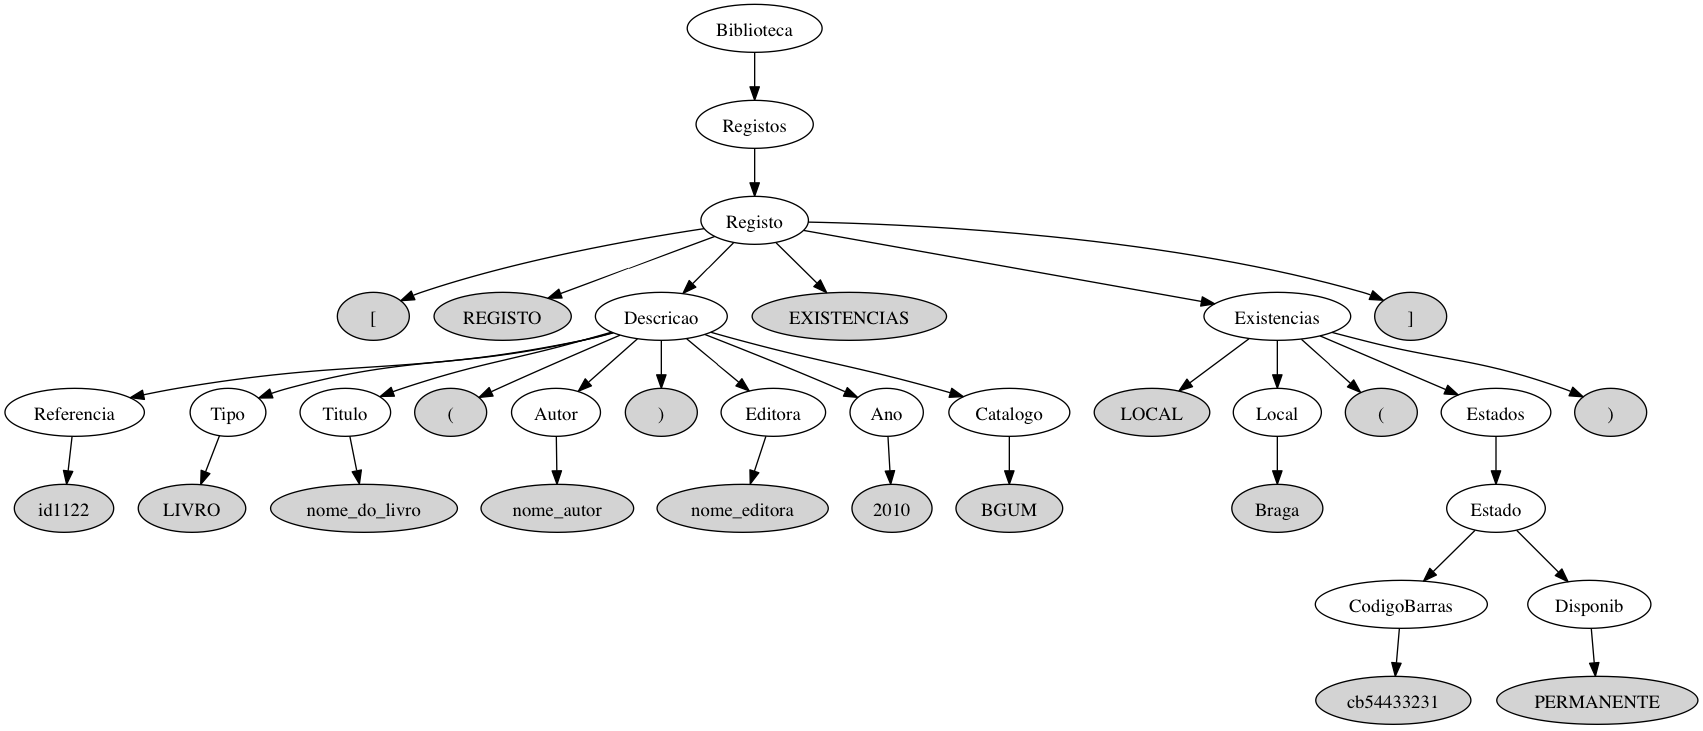
\includegraphics[scale=.33,angle=-90,keepaspectratio]{../ficha5/g.png}
	\end{center}
	\caption{\label{parse_tree_ap}Árvore de Derivação}
\end{figure}

\end{document}
